\documentclass[12pt]{article}

\usepackage[utf8]{inputenc}
\usepackage{datetime}
\usepackage{amsthm}
\usepackage{amsmath}
\usepackage{amssymb}
\usepackage{enumitem}
\usepackage[USenglish]{babel}
\usepackage{matlab-prettifier}
\usepackage{graphicx}

\newcommand\independent{\protect\mathpalette{\protect\independenT}{\perp}}
\def\independenT#1#2{\mathrel{\rlap{$#1#2$}\mkern2mu{#1#2}}}

\newtheoremstyle{colon}{\topsep}{\topsep}{}{}{\bfseries}{:}{ }{}
\theoremstyle{colon}
\newtheorem{exercise}{Exercise}
\newtheorem*{answer}{Answer}

\title{ORFE 523: Conic and Convex Optimization \\ Homework 1}
\author{Zachary Hervieux-Moore}

\newdate{date}{23}{02}{2017}
\date{\displaydate{date}}

\begin{document}

\maketitle

\clearpage

\begin{exercise}
  The singular value decomposition of $A$ is defined as
  \begin{gather*}
    A = U \Sigma V^T
  \end{gather*}
  Where $U, \Sigma, V$ are respectively $m \times m, m \times n, n \times n$. $U$ and $V$ are orthogonal matrices ($U^T U = V^T V = I$). $\Sigma$ is a matrix with $r$ positive scalars $\sigma_1, \mathellipsis, \sigma_r$ on the diagonal of its upper left $r \times r$ block. These are called the \textit{singular values} of $A$ and are given by
  \begin{gather*}
    \sigma_i = \sqrt{i^{th} \text{ eigenvalue of } A^T A}
  \end{gather*}
  By convention, $\sigma_1 \geq \sigma_2 \geq \mathellipsis \geq \sigma_r$. The columns of $U$ and $V$ are the orthonormal eigenvectors of $A A^T$ and $A^T A$.

  \begin{enumerate}[label=\arabic*)]
    \item
      \begin{enumerate}[label=\alph*)]
        \item Show that the eigenvalues of $A^T A$ are always nonnegative. (Hence singular values are well-defined as real, nonnegative scalars.)
        \item Show that if $A$ is a symmetric then the singular values of $A$ are the same as the absolute value of the eigenvalues of $A$.
        \item Show that if $u_i$ and $u_j$ are eigenvectors of $A^T A$ associated with distinct eigenvalues $\lambda_i, \lambda_j$ then $u_i$ and $u_j$ are orthogonal.
      \end{enumerate}

    \item Show that
      \begin{gather*}
        A_{(k)} = \min_{B \in \mathbb{R}^{m \times n}, rank(B) \leq k} \lVert A - B \rVert_2
      \end{gather*}
      Where $A_{(k)} := U_{(k)} \Sigma_{(k)} V_{(k)}^T$. Where $\lVert \cdot \rVert_2$ is the spectral norm defined as $\lVert C \rVert_2 = \max_{\lVert x \rVert_2 = 1} \lVert C x \rVert_2$.

    \item For $k = 25, 50, 100, 150$, use Matlab to compute $A_{(k)}$ as defined above. Report the value of $\lVert A - A_{(k)} \rVert_F$ in each case. (Include your code for this part and the next.)

    \item Use the commands \texttt{subplot} and \texttt{imshow} to produce on the same figure the original image, as well as your compressed images $A_{(k)}$ for $k = 25, 50, 100, 150$. Label your subplots. In addition, produce two separate plots demonstrating (i) $\lVert A - A_{(k)} \rVert_F$ versus $k$, and (ii) ``total savings'' versus $k$. Total savings is to be interpreted as the answer to the question: How many fewer numbers do you need in order to store $A_{(k)}$ than you did to store $A$? Explain why this number is equal to $mn - (n+m+1)k$. How much are you saving for $k = 150$.

    \item Use the Matlab function \texttt{imwrite} to create two images from \texttt{imshow(A)} and \texttt{imshow($\text{A}_{(200)}$)}. Can you tell them apart? Does Shams Tabrizi look any less mystical?
  \end{enumerate}
\end{exercise}

\begin{answer}
  \leavevmode
  \begin{enumerate}[label=\arabic*)]
    \item
      \begin{enumerate}[label=\alph*)]
        \item We have that $A^T A$ is psd since
          \begin{gather*}
            x^T A^T A x = \lVert A x \rVert^2 \geq 0
          \end{gather*}
          Thus, all the eigenvalues must be nonnegative since it is psd.

        \item $A$ is symmetric so $A = A^T$. Thus, $A^T A = A^2$. We now show that an eigenvector of $A$ is an eigenvector of $A^2$.
          \begin{gather*}
            A^2 u = A (A u) = A(\lambda u) = \lambda A u = \lambda^2 u
          \end{gather*}
          Thus the eigenvalues of $A^T A$ are the eigenvalues of $A$ squared. The singular values are then $\sqrt{\lambda_i^2} = \lvert \lambda_i \rvert$.

        \item We will show that $u_i$ is precisely the $i^{th}$ column of $V^T$. First note that
          \begin{gather*}
            A^T A = V \Sigma^2 V^T
          \end{gather*}
          Now, right multiply by the $i^{th}$ column of $V^T$ and use unitarity,
          \begin{gather*}
            V \Sigma^2 V^T V_i = V \Sigma^2 e_i = V \sigma_i^2 e_i = \lambda_i V e_i = \lambda_i V_i
          \end{gather*}
          Thus, if $v_i$ and $v_j$ have distinct eigenvalues, then they are distinct columns of $V^T$. Hence, they are orthogonal.
      \end{enumerate}

    \item We first show that the spectral norm is unitarily invariant. By definition,
      \begin{gather*}
        \lVert A \rVert_2 = \max_{\lVert x \rVert_2 = 1} x^T A^T A x
      \end{gather*}
      Then,
      \begin{gather*}
        \lVert U A \rVert_2 = \max_{\lVert x \rVert_2 = 1} \lVert U A x \rVert_2 \\
        = \max_{\lVert x \rVert_2 = 1} x^T A^T U^T U A x \\
        = \max_{\lVert x \rVert_2 = 1} x^T A^T A x
      \end{gather*}
      Thus, invariant on the left. Now the right,
      \begin{gather*}
        \lVert A V \rVert_2 = \max_{\lVert x \rVert_2 = 1} \lVert A V x \rVert_2 \\
        = \max_{\lVert x \rVert_2 = 1} x^T V^T A^T A V x \\
        = \max_{\lVert y \rVert_2 = 1} y^T A^T A y
      \end{gather*}
      Where $y = V x$ is a one-to-one transformation and $\lVert y \rVert_2 = \lVert x \rVert_2$ because $V$ is unitary. Hence, the spectral norm is unitarily invariant. Now, we develop a lower bound. Suppose that $x \in \text{span}(v_1, \mathellipsis, v_{k+1})$, that is, in the span of the first $k+1$ right singular vectors. Now, since $B$ is of rank $k$, then $\text{null}(B) \bigcap \text{span}(v_1, \mathellipsis, v_{k+1}) \neq \{0\}$. Thus, pick $x$ such that it is in this intersection and its norm is 1. Then
      \begin{gather*}
        \lVert (A - B) x \rVert_2 = \lVert Ax + 0 \rVert_2 = \lVert A x \rVert_2
      \end{gather*}
      Now, since $x$ is a span of singular vectors,
      \begin{gather*}
        = \sqrt{\sum_{i=1}^{k+1} \sigma_i^2 (v_i^T x)^2} \\
        \geq \sigma_{k+1} \cdot \sqrt{\sum_{i=1}^{k+1} (v_i^T x)^2} = \sigma_{k+1}
      \end{gather*}
      Now, we show that $\sigma_{k+1}$ is achieved by $A_{(k)}$. Using unitary invariance,
      \begin{gather*}
        \lVert A - A_{(k)} \rVert_2 \\
        = \lVert U^T A V - U^T U_{(k)} \Sigma_{(k)} V_{(k)}^T V \rVert_2 \\
        = \lVert \Sigma - I_{(k)} \Sigma_{(k)} I_{(k)} \rVert_2 \\
        = \lVert \Sigma - \Sigma_{k} \rVert_2
      \end{gather*}
      Where $I_{(k)}$ is the $n \times n$ identity with only the top first $k$ columns. Now, $\Sigma - \Sigma_{k}$ is simply the singular value matrix with only $\sigma_{k+1}, \mathellipsis, \sigma_r$ on the diagonal. Thus, the spectral norm is $\sigma_{k+1}$. This is precisely our lower bound and so we conclude that $A_{(k)}$ is the solution.

    \item The code used to generate all parts is attached at the end of the question. For this part, the Frobenius norms calculated are shown in Table 1.
      \begin{table}[ht]
        \begin{center}
          \begin{tabular}{ | c | c | c | c | c | }
            \hline
            $k$ & 25 & 50 & 100 & 150 \\
            \hline
            $\lVert A - A_{(k)} \rVert_F$ & 107.99 & 87.55 & 61.46 & 46.39 \\
            \hline
          \end{tabular}
        \end{center}
        \caption{Frobenius norms for various $k$-rank approximations}
      \end{table}

    \item Below are all the figures. For the Figure 1, the image has been scaled down, so it is difficult to see the progression of the lossy compression. The $k$ values are increasing left to right with the original on the furthest right. One can see the difference from $k = 25$ to $k = 150$ as the image becomes less ``fuzzy''. However, the difference between $k = 150$ and the original is quite small and mostly noticeable around the signature. Figure 2 shows how the Frobenius norm changes with $k$. Finally, Figure 3 shows the savings. Notice that around $k = 400$ the savings go negative. That is, you are now using more numbers than the original representation. The savings $mn - (n + m + 1)k$ comes from the fact that $U_{(k)}$ is $m \times k$, $\Sigma_{(k)}$ only needs $k$ numbers on the diagonal (everything else is 0), and $U_{(k)}$ is $n \times k$. Thus, the savings are $mn - mk - k - nk$ or $mn - (n + m + 1)k$. For $k = 150$, you are saving 517482 numbers.
      \begin{figure}[ht]
        \caption{Compressed images for various $k$}
        \centering
          
\includegraphics[width=\textwidth]{part4.jpg}
      \end{figure}

      \begin{figure}[ht]
        \caption{Frobenius norm as $k$ changes}
        \centering
          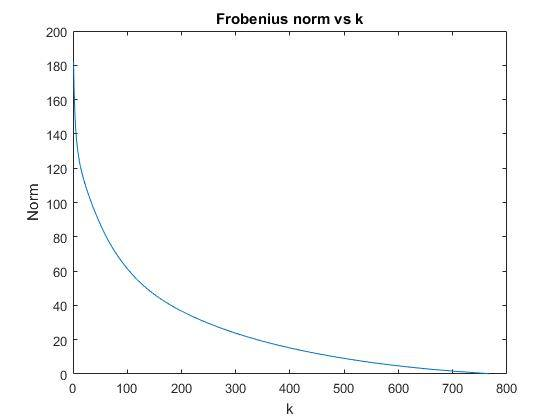
\includegraphics[width=\textwidth]{norm.jpg}
      \end{figure}

      \begin{figure}[ht]
        \caption{Compressed images savings as $k$ varies}
        \centering
          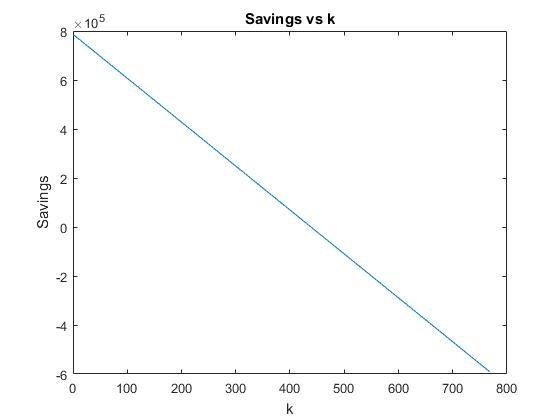
\includegraphics[width=\textwidth]{savings.jpg}
      \end{figure}

    \clearpage

    \item Figure 4 shows the comparison of $A_{(200)}$ and the original. When I look at them, I can only tell the difference near the writting on the left side. As for Shams himself, he is not missing an iota of his mytique.
      \begin{figure}[ht]
        \caption{$A_{(200)}$ on the left and $A$ on the right}
        \centering
          
\includegraphics[width=\textwidth]{part5.jpg}
      \end{figure}
  \end{enumerate}

  \textbf{Code Appendix}

  \begin{lstlisting}[style=Matlab-editor, basicstyle=\scriptsize]
    % Part 3

    clear;
    clc;

    A = imread('Shams.jpg');
    A = im2double(A);
    A = rgb2gray(A);

    [U,S,V] = svd(A);

    m = 768;
    n = 1024;

    figure

    values = [25,50,100,150];
    for i = 1:length(values)
        % Calculate A_k
        k = values(i);
        U_k = U(:,1:k);
        S_k = S(1:k,1:k);
        V_k = V(:,1:k);
        A_k = U_k*S_k*V_k';

        % Calculate Frobenius norm
        norm(A - A_k,'fro')

        subplot(1,5,i);
        imshow(A_k)
        title(['k = ', num2str(k)]);
    end

    subplot(1,5,5);
    imshow(A_k)
    title('Original');

    % Part 4

    for k = 1:768
        % Calculate A_k
        U_k = U(:,1:k);
        S_k = S(1:k,1:k);
        V_k = V(:,1:k);
        A_k = U_k*S_k*V_k';

        % Calculate Frobenius norm
        result(k) = norm(A - A_k,'fro');
        savings(k) = m*n - (n+m+1)*k;
    end

    figure
    plot(result);
    title('Frobenius norm vs k');
    ylabel('Norm');
    xlabel('k');

    figure
    plot(savings);
    title('Savings vs k');
    ylabel('Savings');
    xlabel('k');

    savings(150)

    % Part 5

    k = 200;
    U_k = U(:,1:k);
    S_k = S(1:k,1:k);
    V_k = V(:,1:k);
    A_k = U_k*S_k*V_k';

    figure
    subplot(1,2,1);
    imshow(A_k)
    title('A_{200}');

    subplot(1,2,2);
    imshow(A)
    title('Original');
  \end{lstlisting}
\end{answer}

\clearpage

\begin{exercise}
  Let
  \begin{gather*}
    f(x_1, x_2) = \frac{1}{3} x_1^3 - \frac{1}{2} x_1^2 + 2 x_1 x_2 + \frac{1}{2} x_2^2
  \end{gather*}

  \begin{enumerate}[label=\arabic*)]
    \item Find the local and global minimizers of this function.

    \item Without using arguments based on convexity, prove that for any quad-ratic function $f(x) = x^T Q x + b^T x + c$, the following statements hold:
    \begin{enumerate}[label=\alph*)]
      \item $\bar{x}$ is a local min $\nabla f(\bar{x}) = 0$ and $\nabla^2 f(\bar{x}) \succeq 0$.
      \item$\bar{x}$ is a strict local min $\nabla f(\bar{x}) = 0$ and $\nabla^2 f(\bar{x}) \succ 0$.
    \end{enumerate}
    Give counterexamples to show that these statements are not true for twice differentiable functions in general.

    \item The rate of increase of a function $f: \mathbb{R}^n \rightarrow \mathbb{R}$ at a point $x$ and in a nonzero direction $d$ is given by $g'(0)$, where $g: \mathbb{R} \rightarrow \mathbb{R}$ is defined as
      \begin{gather*}
        g(\alpha) = f \left( x + \alpha \frac{s}{\lVert d \rVert} \right)
      \end{gather*}
      Show that the minimum and maximum rates of increase are achieved in the directions $- \nabla f(x)$ and $\nabla f(x)$ respectively.
  \end{enumerate}
\end{exercise}

\begin{answer}
  \leavevmode
  \begin{enumerate}[label=\arabic*)]
    \item First, we find the critical points by setting the gradient to 0.
      \begin{gather*}
        \nabla f(x) = \begin{bmatrix}
          x_1^2 - x_1 + 2 x_2 \\
          2 x_1 + x_2
        \end{bmatrix} = \begin{bmatrix}
          0 \\
          0
        \end{bmatrix}
      \end{gather*}
      The second entry gives us $x_2 = -2 x_1$. Which, when substituted back into the first entry, gives $x_1 (x_1 - 5) = 0$. Thus, we have two candidate points. $(0,0)$ and $(5, -10)$. The Hessians for $f$ is
      \begin{gather*}
        H(f)(x) = \begin{bmatrix}
          2 x_1 - 1 && 2 \\
          2 && 1
        \end{bmatrix}
      \end{gather*}
      Thus, the Hessian at the two critical points are
      \begin{gather*}
        H(f)(x) = \begin{bmatrix}
          -1 && 2 \\
          2 && 1
        \end{bmatrix} \text{ and } \begin{bmatrix}
          9 && 2 \\
          2 && 1
        \end{bmatrix}
      \end{gather*}
      Notice that the first Hessian is indefinite (pick $(1,0)$ and $(0,1)$). Where the second one is positive definite since the leading principal minors are all positive. Thus, we have that $(5, -10)$ is a strict local min. Notice that there are no global minimums or maximums because setting $x_2 = 0$ and letting $x_1 \rightarrow \pm \infty$ will yield an arbitrary high or low value.

    \item We first write the Taylor series at $\bar{x}$. Note that there are no terms of degree higher than 2 because the derivatives of the quadratic are all 0 (the Lagrange remainder is 0).
      \begin{gather*}
        f(x) = f(\bar{x}) + \nabla f(\bar{x})^T (\bar{x} - x) + (\bar{x} - x)^T Q (\bar{x} - x)
      \end{gather*}
      \begin{enumerate}[label=\alph*)]
        \item The backwards implication goes as follows. If $\nabla f(\bar{x}) = 0$ then
          \begin{gather*}
            f(x) = f(\bar{x}) + (\bar{x} - x)^T Q (\bar{x} - x)
          \end{gather*}
          If $Q \succeq 0$, then going $\epsilon$ in any direction $d$ yields.
          \begin{gather*}
            f(\bar{x} + \epsilon d) = f(\bar{x}) + (\epsilon d)^T Q (\epsilon d) \geq f(\bar{x})
          \end{gather*}
          Thus, we have have a local minimum. For the forward implication, assume we have a local min. Then $f(\bar{x} + \epsilon d) \geq f(\bar{x})$. Thus, we have
          \begin{gather*}
            f(\bar{x} + \epsilon d) = f(\bar{x}) - \nabla f(\bar{x})^T (\epsilon d) + (\epsilon d)^T Q (\epsilon d) \geq f(\bar{x})
          \end{gather*}
          Now, if $\nabla f(\bar{x}) \neq 0$ then we can pick $d$ to target the non-zero entry of $\nabla f(\bar{x})$ and make it positive. Call this entry $i$. That is $d = (0,\mathellipsis,1,0,\mathellipsis,0)$ if $f(\bar{x})_i > 0$ or $d = (0,\mathellipsis,-1,0,\mathellipsis,0)$ if $f(\bar{x})_i < 0$. Furthermore, the quadratic term will become $\epsilon^2 Q_{ii}$. So we have
          \begin{gather*}
            f(\bar{x} + \epsilon d) = f(\bar{x}) - \epsilon \lvert \nabla f(\bar{x})_i \rvert + \epsilon^2 Q_{ii} \geq f(\bar{x})
          \end{gather*}
          However, we can pick $\epsilon$ sufficiently small so that $\epsilon \lvert \nabla f(\bar{x})_i \rvert > \epsilon^2 Q_{ii}$. This will yield
          \begin{gather*}
            f(\bar{x} + \epsilon d) = f(\bar{x}) - \epsilon \lvert \nabla f(\bar{x})_i \rvert + \epsilon^2 Q_{ii} < f(\bar{x})
          \end{gather*}
          Which contradicts our assumption that $\bar{x}$ is a local min. Thus, we must have that $\nabla f(\bar{x}) = 0$. With this constraint, we have the Taylor expansion
          \begin{gather*}
            f(\bar{x} + \epsilon d) = f(\bar{x}) + (\epsilon d)^T Q (\epsilon d)
          \end{gather*}
          Now, for this to be greater than or equal to $f(\bar{x})$. We need $(\epsilon d)^T Q (\epsilon d) \geq 0$ for all $d$. Hence, we need $Q$ to be positive semidefinite.

          A counterexample in $C^2$ to this statement is $f(x) = x^3$. We have that $\nabla f(0) = 0$ and $\nabla^2 f(0) = 0$ but $f(0)$ is not a local min since $f(-\epsilon) = -\epsilon^3 < 0$.

        \item The proof of this statement is nearly identical to the previous up to changes inequalities. The backwards implication goes as follows. If $\nabla f(\bar{x}) = 0$ then
          \begin{gather*}
            f(x) = f(\bar{x}) + (\bar{x} - x)^T Q (\bar{x} - x)
          \end{gather*}
          If $Q \succ 0$, then going $\epsilon$ in any direction $d$ yields.
          \begin{gather*}
            f(\bar{x} + \epsilon d) = f(\bar{x}) + (\epsilon d)^T Q (\epsilon d) > f(\bar{x})
          \end{gather*}
          Thus, we have have a strict local minimum. For the forward implication, assume we have a strict local min. Then $f(\bar{x} + \epsilon d) > f(\bar{x})$. Thus, we have
          \begin{gather*}
            f(\bar{x} + \epsilon d) = f(\bar{x}) - \nabla f(\bar{x})^T (\epsilon d) + (\epsilon d)^T Q (\epsilon d) > f(\bar{x})
          \end{gather*}
          Now, if $\nabla f(\bar{x}) \neq 0$ then we can pick $d$ to target the non-zero entry of $\nabla f(\bar{x})$ and make it positive. Call this entry $i$. That is $d = (0,\mathellipsis,1,0,\mathellipsis,0)$ if $f(\bar{x})_i > 0$ or $d = (0,\mathellipsis,-1,0,\mathellipsis,0)$ if $f(\bar{x})_i < 0$. Furthermore, the quadratic term will become $\epsilon^2 Q_{ii}$. So we have
          \begin{gather*}
            f(\bar{x} + \epsilon d) = f(\bar{x}) - \epsilon \lvert \nabla f(\bar{x})_i \rvert + \epsilon^2 Q_{ii} > f(\bar{x})
          \end{gather*}
          However, we can pick $\epsilon$ sufficiently small so that $\epsilon \lvert \nabla f(\bar{x})_i \rvert > \epsilon^2 Q_{ii}$. This will yield
          \begin{gather*}
            f(\bar{x} + \epsilon d) = f(\bar{x}) - \epsilon \lvert \nabla f(\bar{x})_i \rvert + \epsilon^2 Q_{ii} < f(\bar{x})
          \end{gather*}
          Which contradicts our assumption that $\bar{x}$ is a strict local min. Thus, we must have that $\nabla f(\bar{x}) = 0$. With this constraint, we have the Taylor expansion
          \begin{gather*}
            f(\bar{x} + \epsilon d) = f(\bar{x}) + (\epsilon d)^T Q (\epsilon d)
          \end{gather*}
          Now, for this to be always greater than $f(\bar{x})$. We need \\ $(\epsilon d)^T Q (\epsilon d) > 0$ for all $d \neq 0$. Hence, we need $Q$ to be positive definite.

          A counterexample of this statement in $C^2$ is $f(x) = x^4$. We have that $x = 0$ is a strict local min since $f(\pm \epsilon) = \epsilon^4 > 0$. However, $\nabla^2 f(0) = 0$ which is not positive definite.
      \end{enumerate}

      \item First, lets write out $g'(0)$. This is equal to
        \begin{gather*}
          g'(\alpha) = \frac{d^T}{\lVert d \rVert} \nabla f \left(x + \alpha \frac{d}{\lVert d \rVert} \right) \\
          g'(0) = \frac{d^T}{\lVert d \rVert} \nabla f(x)
        \end{gather*}
        Now we apply Cauchy-Schwarz inequality
        \begin{gather*}
          \lvert \langle u, v \rangle \rvert \leq \lVert u \rVert \lVert v \rVert \\
          \Longleftrightarrow -\lVert u \rVert \lVert v \rVert \leq \langle u, v \rangle \leq \lVert u \rVert \lVert v \rVert
        \end{gather*}
        Applied to our problem,
        \begin{gather*}
          -\lVert \frac{d}{\lVert d \rVert} \rVert \lVert \nabla f(x) \rVert \leq \frac{d^T}{\lVert d \rVert} \nabla f(x) \leq \lVert \frac{d}{\lVert d \rVert} \rVert \lVert \nabla f(x) \rVert
        \end{gather*}
        However, $\lVert \frac{d}{\lVert d \rVert} \rVert = 1$. Which simplifies to
        \begin{gather*}
          -\lVert \nabla f(x) \rVert \leq \frac{d^T}{\lVert d \rVert} \nabla f(x) \leq \lVert \nabla f(x) \rVert
        \end{gather*}
        Now, picking $d = \nabla f(x)$ will result in the upper bound and choosing $d = - \nabla f(x)$ results in the lower bound. Thus, we conclude that the minimum and maximum rates of increase are achieved in the directions $-\nabla f(x)$ and $\nabla f(x)$ respectively.
  \end{enumerate}
\end{answer}

\clearpage

\begin{exercise}
  \leavevmode
  \begin{enumerate}[label=\arabic*)]
    \item Let $Q \in S^{n \times n}$ and assume $Q \succ 0$. Show that
      \begin{gather*}
        f(x) = \sqrt{ x^T Q x}
      \end{gather*}
      is a norm.

    \item Show that $Q^{-1}$ exists and is positive definite. Show that the dual norm of $f$ is given by
      \begin{gather*}
        g(x) = \sqrt{x^T Q^{-1} x}
      \end{gather*}
      (Hint: You may want to bring in $\sqrt{Q}$, i.e., a matrix whose square is $Q$. If you do, you have to first prove that this matrix exists.)

    \item Let $A \in \mathbb{R}^{m \times n}$. Proce the following expression for its induces 2-norm:
      \begin{gather*}
        \lVert A \rVert = \sqrt{\lambda_{\text{max}}(A^T A)}
      \end{gather*}
  \end{enumerate}
\end{exercise}

\begin{answer}
  \leavevmode
  \begin{enumerate}[label=\arabic*)]
    \item We will show that $\langle x, y \rangle = x^T Q y$ is an inner product which necessitates that $\sqrt{\langle x,x \rangle} = f(x)$ is a norm.
      \begin{enumerate}[label=\roman*)]
        \item Positivity: $\langle x, x \rangle = x^T Q x \geq 0$ since $Q \succ 0$. Furthermore, since $Q$ is positive definite, it only equals 0 when $x = 0$.

        \item Symmetry: $\langle x, y \rangle$ is a scalar. Hence, it is equal to its transpose.
          \begin{gather*}
            \langle x, y \rangle = x^T Q y = y^T Q x = \langle y, x \rangle
          \end{gather*}

        \item Additivity: This results from distributivity of matrix multiplication.
          \begin{gather*}
            \langle x + y, z \rangle = (x+y)^T Q z = x^T Q z + y^T Q z = \langle x, z \rangle + \langle y, z \rangle
          \end{gather*}

        \item Homogeneity: Also a result of matrices. Let$ \alpha \in \mathbb{R}$.
          \begin{gather*}
            \langle \alpha x, y \rangle = (\alpha x)^T Q y = \alpha(x^T Q y) = \alpha \langle x, y \rangle
          \end{gather*}
      \end{enumerate}
      Thus, $\langle x,y \rangle$ is an inner product so $f(x)$ is a norm.

    \item As per the hint, we show that $\sqrt{Q}$ exists where $\sqrt{Q}^2 = Q$. Since $Q$ is real symmetric, it has a decomposition of $P$ and $\Lambda$ where $P$ is orthonormal and $\Lambda$ is diagonal. I.e., $Q = P^T \Lambda P$. We now define $\sqrt{\Lambda}$ as the matrix of taking square roots of the diagonal matrix $\Lambda$. Thus we have
      \begin{gather*}
        (P^T \sqrt{\Lambda} P)^2 = P^T \sqrt{\Lambda} P P^T \sqrt{\Lambda} P \\
        = P^T \sqrt{\Lambda} I \sqrt{\Lambda} P \\
        = P^T \sqrt{\Lambda} \sqrt{\Lambda} P \\
        = P^T \Lambda P = Q
      \end{gather*}
      Thus, $\sqrt{Q}$ exists and is precisely given by $P^T \sqrt{\Lambda} P$. Furthermore, $\sqrt{Q}$ is also symmetric. Now, we write the norm $f(x)$ as
      \begin{gather*}
        f(x) = \sqrt{x^T \sqrt{Q} \sqrt{Q} x} = \sqrt{x^T \sqrt{Q}^T \sqrt{Q} x} = \lVert \sqrt{Q} x \rVert_2
      \end{gather*}
      That is, the matrix norm is equivalent to this weighted vector norm. We now find the dual of this new (but equivalent) norm.
      \begin{gather*}
        \max_{s.t. \lVert \sqrt{Q} y \rVert_2 \leq 1} x^T y
      \end{gather*}
      But, we can use a change of variable $z = \sqrt{Q} y$ or $y = \sqrt{Q}^{-1} z$. Note that $Q^{-1}$ exists since $Q$ is positive definite, then the decomposition we used before has no 0 entries on the diagonal of $\Lambda$ (the diagonal is precisely the eigenvalues of $Q$). Thus, the inverse is defined to be $P^T \Lambda^{-1} P$ where $\Lambda^{-1}$ is simply the same as $\Lambda$ but with the entries inverted. Thus,
      \begin{gather*}
        Q Q^{-1} = P^T \Lambda P P^T \Lambda^{-1} P = P^T \Lambda \Lambda^{-1} P = P^T P = I
      \end{gather*}
      We then define $\sqrt{Q}^{-1}$ as before but for $Q^{-1}$. Now, our norm becomes
      \begin{gather*}
        \max_{s.t. \lVert z \rVert_2 \leq 1} x^T \sqrt{Q}^{-1} z
      \end{gather*}
      Which we know from the notes is achieved when $z = \frac{\sqrt{Q}^{-1} x}{\lVert \sqrt{Q}^{-1} x \rVert_2}$. Hence, the dual norm is
      \begin{gather*}
        g(x) = \frac{x^T \sqrt{Q}^{-1} \sqrt{Q}^{-1} x}{\sqrt{x^T \sqrt{Q}^{-1} \sqrt{Q}^{-1} x}} \\
        = \frac{x^T Q^{-1} x}{\sqrt{x^T Q^{-1} x}} \\
        = \sqrt{x^T Q^{-1} x}
      \end{gather*}
      Which is the result desired.

    \item First, the induced 2-norm is
      \begin{gather*}
        \max_{s.t. \lVert x \rVert_2 \leq 1} \lVert A x \rVert_2 = \max_{s.t. \lVert x \rVert_2 \leq 1} \sqrt{x^T A^T A x}
      \end{gather*}
      Now, $A^T A$ is real symmetric, so we can use the same decomposition as before. $A^T A = P^T \Lambda P$ where $\Lambda$ are the eigenvalues of $A^T A$ and $P$ is orthonormal. Thus, the norm is
      \begin{gather*}
        = \max_{s.t. \lVert x \rVert_2 \leq 1} \sqrt{x^T P^T \Lambda P x}
      \end{gather*}
      But, since $P$ is orthonormal, then $y = P x$ has the same norm. So, we perform this change of variable with no change in the constraint.
      \begin{gather*}
        = \max_{s.t. \lVert y \rVert_2 \leq 1} \sqrt{y^T \Lambda y}
      \end{gather*}
      Since, $\Lambda$ is diagonal, we pick $y = e_i$ such that it picks the largest element on the diagonal of $\Lambda$. This corresponds to the largest eigenvalue of $A^T A$. Thus, the induced norm becomes
      \begin{gather*}
        = \sqrt{y^T \Lambda y} = \sqrt{e_i \Lambda e_i} = \sqrt{\lambda_{\text{max}} (A^T A)}
      \end{gather*}
  \end{enumerate}
\end{answer}

\clearpage

\begin{exercise}
  Prove or disprove the following statements. All matrices are $n \times n$ and with real entries.
  \begin{enumerate}[label=\alph*)]
    \item Suppose $A \succeq 0$. Then the largest entry in absolute value of $A$ must be on the diagonal.
    \item If $A \succeq 0$ and trace($A$) = 0, then $A = 0$.
    \item If $A \succeq 0$, $B \succeq 0$, and $A+B = 0$, then $A = B = 0$.
    \item If $A \succeq 0$, $B \succeq 0$, and $AB = 0$, then $A = 0$ or $B = 0$.
  \end{enumerate}
\end{exercise}

\begin{answer}
  \leavevmode
  \begin{enumerate}[label=\alph*)]
    \item Suppose that the largest element is not located on the diagonal. Suppose at $A_{ij}$. Then pick the vector $v = (0,\mathellipsis,0,1,0,\mathellipsis,0,-1,0,\mathellipsis,0)$. Where the 1 is at index $i$ and the $-1$ at index $j$. If $A_{ij}$ is negative then use two positive 1's. We assume it is positive. Then we have
    \begin{gather*}
      v^T A v = \sum_{i,j = 1}^n v_i A_{ij} v_j = A_{ii} + A_{jj} - 2A_{ij}
    \end{gather*}
    However, this matrix is psd thus
    \begin{gather*}
      A_{ii} + A_{jj} - 2A_{ij} \geq 0 \\
      A_{ii} + A_{jj} \geq 2 A_{ij}
    \end{gather*}
    However, if $A_{ij}$ is the largest element, then
    \begin{gather*}
      2 A_{ij} > A_{ii} + A_{jj}
    \end{gather*}
    Which contradicts the assumption that $A$ is psd.

    \item Since $A \succeq 0$, then the diagonal is nonnegative. If trace($A$) = 0, then this must mean that the diagonal elements are all 0 since you are summing nonnegative elements. By part a), the largest absolute value appears on the diagonal. However, the entire diagonal is 0 and hence the entire matrix must be 0. That is, $A = 0$.

    \item If $A + B = 0$, then we have trace($A$) + trace($B$) = 0. Since both matrices are psd, their diagonals must be nonnegative. Thus, we must have trace($A$) = trace($B$) = 0. It follows from part b) that $A = B = 0$.

    \item A counterexample is
      \begin{gather*}
        A = \begin{bmatrix}
          1 && -1 \\
          -1 && 1
        \end{bmatrix} \text{ and } B = \begin{bmatrix}
          1 && 1 \\
          1 && 1
        \end{bmatrix}
      \end{gather*}
      It is easily verified that $A$ and $B$ are psd by Sylvester's criterion (in fact, $B$ is positive definite). However, $AB = 0$.
  \end{enumerate}
\end{answer}

\clearpage

\begin{exercise}
  A $n \times n$ real symmetric matrix $Q$ is said to be \textit{copositive} if $x^T Q x \geq 0$ for all $x \in \mathbb{R}^n$ such that $x \geq 0$. (The inequality on $x$ is elementwise.)
  \begin{enumerate}[label=\alph*)]
    \item Prove that the set of $n \times n$ copositive matrices is convex. Show that the set of $n \times n$ noncopositive matrices is nonconvex unless $n = 1$.
    \item Give an example of a matrix that is copositive but neither positive semidefinite nor elementwise nonnegative. (You have to proves all claims about the example that you produce.)
  \end{enumerate}
\end{exercise}

\begin{answer}
  \leavevmode
  \begin{enumerate}[label=\alph*)]
    \item We first show that the set of copositive matrices is convex. Let $A$ and $B$ be copositive matrices and $\lambda \in (0,1)$. Then we have
      \begin{gather*}
        x^T (\lambda A + (1-\lambda)B) x = \lambda x^T A x + (1-\lambda) x^T B x
      \end{gather*}
      However, by copositive, we have $x^T A x \geq 0$ and $x^T B x \geq 0$. As well, $\lambda > 0$ and $(1-\lambda > 0)$. Thus, all the terms are nonnegative. Thus, we conclude
      \begin{gather*}
        x^T (\lambda A + (1-\lambda)B) x = \lambda x^T A x + (1-\lambda) x^T B x \geq 0
      \end{gather*}
      Therefore, $\lambda A + (1-\lambda)B$ is copositive and hence the set is convex. Now, to show the set of noncopositive matrices is convex for $n \geq 2$. Let us assume that $A$ and $B$ are all 0 except their upper left $2 \times 2$ blocks are
      \begin{gather*}
        A_{2 \times 2} = \begin{bmatrix}
          -1 && 1 \\
          -1 && 1
        \end{bmatrix} \text{ and } B_{2 \times 2} = \begin{bmatrix}
          1 && -1 \\
          1 && -1
        \end{bmatrix}
      \end{gather*}
      Clearly, these are noncopositive since we have $e_1^T A e_1 = -1 < 0$ and $e_2^T B e_2 = -1 < 0$ where $e_i$ is the canonical basis. Now, by taking a linear combination we have
      \begin{gather*}
        \lambda A_{2 \times 2} + (1-\lambda) B_{2 \times 2} = \begin{bmatrix}
          2 \lambda - 1 && 1 - 2 \lambda \\
          2 \lambda - 1 && 1 - 2 \lambda
        \end{bmatrix}
      \end{gather*}
      Settings $\lambda = 1/2$ yields
      \begin{gather*}
        \frac{1}{2} A_{2 \times 2} + \frac{1}{2} B_{2 \times 2} = \begin{bmatrix}
          0 && 0 \\
          0 && 0
        \end{bmatrix}
      \end{gather*}
      Which is vacuously copositive. Hence, noncopositive matrices are not convex when $n \geq 2$. However, when $n = 1$, then noncopositive means that the numbers belong to $\mathbb{R}_{< 0}$ (since $x^T A x = A x^2$ in one dimension). Thus, picking $a, b \in \mathbb{R}_{< 0}$ and $\lambda \in (0,1)$ results in
      \begin{gather*}
        x (\lambda a + (1-\lambda)b) x = \lambda a x^2 + (1-\lambda) b x^2 < 0
      \end{gather*}
      Which is negative because both terms have exactly one negative term.

    \item A matrix that satisfies these conditions is
      \begin{gather*}
        A = \begin{bmatrix}
          1 && 1 && 0.5 \\
          1 && 1 && -1 \\
          0.5 && -1 && 1
        \end{bmatrix}
      \end{gather*}
      This is clearly not elementwise nonnegative. Also, it is not psd since det($A$) = $-2.25$. To show that it is copositive, we can write $x^T A x$ as follows
      \begin{gather*}
        x^T A x = x_1^2 + (2 x_2 + x_3) x_1 + (x_2 - x_3)^2
      \end{gather*}
      This is a quadratic in $x_1$. Notice that if we fix $x_2, x_3 \geq 0$ then we guarantee $x_1 \geq 0$. This is because the roots of this quadratic are both negative. Anything right of the greater root is positive. The right root occurs at
      \begin{gather*}
        \frac{-(2 x_2 + x_3) +  \sqrt{(2 x_2 + x_3)^2 - 4 (x_2 - x_3)^2}}{2}
      \end{gather*}
      We wish this to be negative. That is, using the typical notation of the quadratic formula, we want $\sqrt{b^2 - 4ac} < b$ as we know $b$ is positive. Since $a = 1$, this simplifies to asking if $c > 0$. We have that $c = (x_2 - x_3)^2$ and hence is always positive (except at the origin). Thus, we have shown that $x^T A x$ is always nonnegative and we conclude that $A$ is copositive.
  \end{enumerate}
\end{answer}

\end{document}